\documentclass[convert]{standalone}
\usepackage{tikz} 
\usetikzlibrary{chains,scopes}
\begin{document}

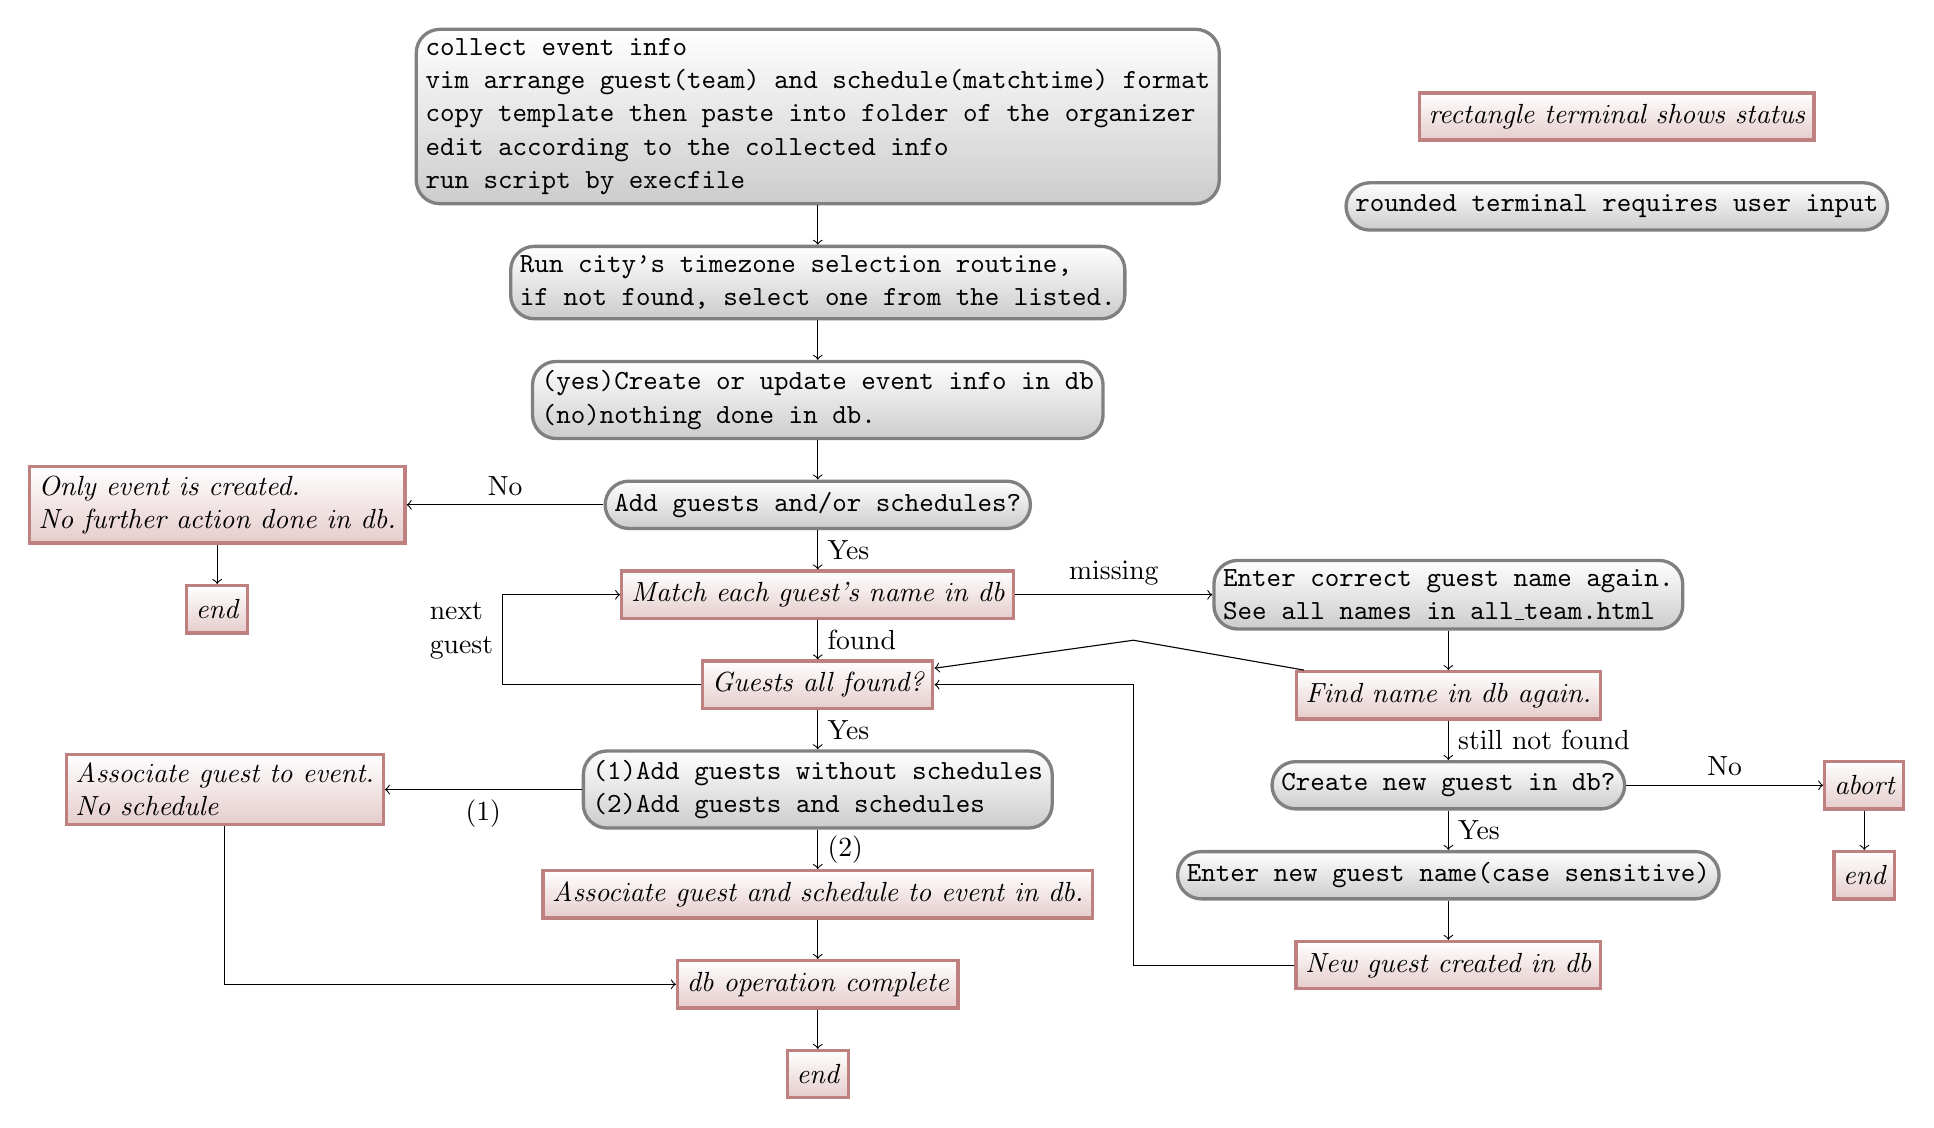
\begin{tikzpicture}[every on chain/.style=join,every join/.style=->,
nonterminal/.style={
	% The shape:
	rectangle,
	% The size:
	minimum size=6mm,
	% The border:
	very thick,
	draw=red!50!black!50, % 50% red and 50% black,
	% and that mixed with 50% white
	% The filling:
	top color=white, % a shading that is white at the top...
	bottom color=red!50!black!20, % and something else at the bottom
	% Font
	font=\itshape},
terminal/.style={
	% The shape:
	rectangle,minimum size=6mm,rounded corners=3mm,
	% The rest
	very thick,draw=black!50,
	top color=white,bottom color=black!20,
	font=\ttfamily},
node distance=0.5cm and 2.5cm,align=left]

%Begin main chain
{ [start chain=trunk going below]
\node (A) [terminal,on chain] {collect event info\\
			vim arrange guest(team) and schedule(matchtime) format\\
			copy template then paste into folder of the organizer\\
			edit according to the collected info\\
			run script by execfile};
\node (AB) [terminal,on chain] {Run city's timezone selection routine,\\
				if not found, select one from the listed.};
\node (B) [terminal,on chain] {(yes)Create or update event info in db\\
					(no)nothing done in db.};
\node (C) [terminal,on chain] {Add guests and/or schedules?};
{ [start branch=event going left] } % just a declaration,
\node (D) [nonterminal,on chain] {Match each guest's name in db};
{ [start branch=team going below] } % we will come back later
\node (E) [nonterminal,on chain] {Guests all found?};
\node (F) [terminal,on chain] {(1)Add guests without schedules\\
			       (2)Add guests and schedules};
{ [start branch=guest going left] } % we will come back later
\node (G) [nonterminal,on chain] {Associate guest and schedule to event in db.};
\node (H) [nonterminal,on chain] {db operation complete};
\node (I) [nonterminal,on chain] {end};

% Now come the branches...
{[continue branch=event]
\node (1) [nonterminal,on chain] {Only event is created.\\
				  No further action done in db.};
\node (2) [nonterminal,on chain=going below] {end};
}
{[continue branch=team]
\node (a) [terminal,on chain=going right] {Enter correct guest name again.\\ See all names in all\_team.html};
\node (b) [nonterminal,on chain] {Find name in db again.};
\node (c) [terminal,on chain] {Create new guest in db?};
{[start branch=abort going right]
	\node (ta)[nonterminal, on chain] {abort};
	\node [nonterminal,on chain=going below] {end};
}
\node (d) [terminal, on chain] {Enter new guest name(case sensitive)};
\node (e) [nonterminal,on chain] {New guest created in db};
}
{[continue branch=guest]
\node (99) [nonterminal,on chain=going left] {Associate guest to event.\\ No schedule};
}
}
%End Chain envr

\draw[->] (e)  -- ++(-4cm,0)  |- (E);
\draw[->] (E) -- ++(-4cm,0)  |- node[pos=0.3,auto] {next\\guest} (D);
\draw[->] (b)  -- ++(-4cm,0.7cm)  -- (E);
\draw[->] (99)  |- (H);

\path (C) -- (1) node[pos=0.5,above] {No};
\path (C) -- (D) node[pos=0.5,auto] {Yes};
\path (D) -- (a) node[pos=0.5,auto] {missing};
\path (D) -- (E) node[pos=0.5,auto] {found};
\path (b) -- (c) node[pos=0.5,auto] {still not found};
\path (c) -- (d) node[pos=0.5,auto] {Yes};
\path (c) -- (ta) node[pos=0.5,auto] {No};
\path (E) -- (F) node[pos=0.5,auto] {Yes};
\path (F) -- (99) node[pos=0.5,auto] {(1)};
\path (F) -- (G) node[pos=0.5,auto] {(2)};

\node (r) [right = of A,nonterminal] {rectangle terminal shows status};
\node[below = of r,terminal] {rounded terminal requires user input};

\end{tikzpicture}

\end{document}
